%%
%%  APPENDICES FOR THE CHAPTER 2
%%
\chapter{Some effects for the zip2 synchroniser}
  \section{One of the channels queues is always empty}
TODO

  \section{Brownian motion in unlimited queues}
Explain why the phenomena is observed for $\langle (n_{a} - n_{b})^{2} \rangle$. Explain the similarity of fluctuations of $n_{a} - n_{b}$ the the Brownian motion.
  \begin{figure}[h!]
  \centering
  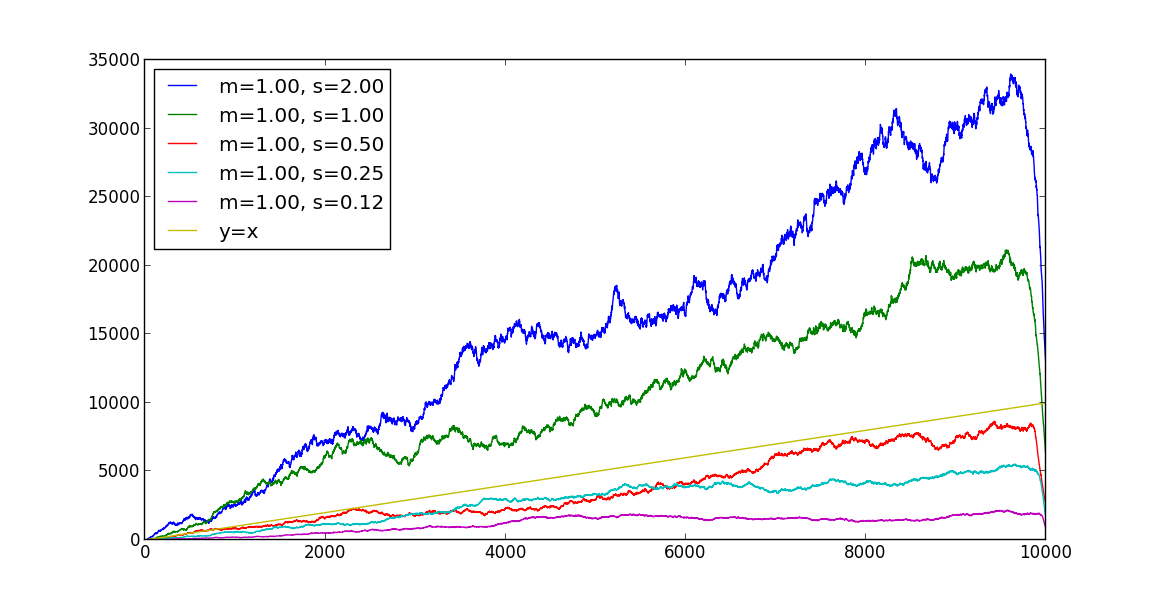
\includegraphics[scale=0.4]{figs/all.png}
  \caption{The evolution of $(n_{a} - n_{b})^{2}$ over time depending on the variance $\sigma$.}
  \label{fig:brownian}
  \end{figure}

Reflected Brownian motion on the half line $[0,\infty$

Brownian motion $\langle (n_{a} - n_{b})^{2} \rangle \sim t$, where $n_{a}$ and $n_{b}$ are the number of messages in the channels $a$ and $b$ respectively, and $t$ is time. The average for $(n_{a} - n_{b})$ is taken for 30 experiments. Dependencies close to the Brownian motion $\bar{\Delta l^2} = 2Dt$ take place with the mass diffusivity $D$ as shown in the table below (Коэффициент определен на глаз. По хорошему надо аппроксимировать до прямой: брать среднее от углов наклона для прямых, проведенных через каждую точку). (Probably need to show that the dependency is linear with some statistical criteria like $\chi^{2}$ ?)
  \begin{tabular}{c|c|c|c}
  $m$ & $\sigma$ & $2D$ & $D$\\
  \hline
  $1$ & $2$ & $4$ & $2$\\
  \hline
  $1$ & $1$ & $2$ & $1$\\
  \hline
  $1$ & $0.5$ & $1$ & $0.5$\\
  \hline
  $1$ & $0.25$ & $0.5$ & $0.25$\\
  \hline
  $1$ & $0.125$ & $0.125$ & $0.125$\\ 
  \end{tabular}

Нужно пересчитать эксперимент для $m \neq 1$. Получается что-то похожее на $D = \frac{\sigma}{m^{2}}$. See \ref{fig:brownian}.

It would be good to find $D$ analiticaly!

  \section{The channel length dependent throughtput formula}
The general case probability matrix is in Table \ref{tbl:zip2_prob_mat}.

In our example we assume that both input channels are the same, i.e. the interarrival time in both channels is distributed according to the same law $Gamma(k,\theta,t_t)$. Then, the probability to see 1 message in the channel $a$ and see no messages in the channel $b$ over the time $t_t$ $P_a = P_b = p(1-p)$, where $p = Gamma(k,\theta,t_t)$ is the probability to see 1 message in a channel over time $t_t$.

$P_{ab} = P_{ba} = \frac{p^2}{2}$ is the probability to see 1 message in the channel $a$ and 1 message in the channel $b$, and $b$ after $a$. the probability to see no messages in the channels over time $t_t$ $P_n = (1-p)^2$.


\begin{sidewaystable}
  %\centering
  % make the table fit onto the page
  \scriptsize
  % stretch the rows in the table
  \def\arraystretch{2}
  \begin{tabular}{c|c|>{\centering\arraybackslash}p{2.1cm}|c|c|c|>{\centering\arraybackslash}p{2.1cm}|c|c|c}
  & $\mathbf{A_0 \: B_0 \: L_0}$ & $\mathbf{A_k \: B_0 \: L_0}$ & $\mathbf{A_{l-1} \: B_0 \: L_1}$ & $\mathbf{A_l \: B_0 \: L_0}$ & $\mathbf{A_l \: B_0 \: L_1}$ & $\mathbf{A_0 \: B_k \: L_0}$ & $\mathbf{A_0 \: B_{l-1} \: L_1}$ & $\mathbf{A_0 \: B_l \: L_0}$ & $\mathbf{A_0 \: B_l \: L_1}$\\
  \hline
  $\mathbf{A_0 \: B_0 \: L_0}$ & $P_n+P_{ab}+P_{ba}$ & $P_a \: (k=1)$ & 0 & 0 & 0 & $P_b \: (k=1)$ & 0 & 0 & 0\\
  \hline
  $\mathbf{A_j \: B_0 \: L_0}$ & $P_b \: (j=1)$ & $P_a \: (k-j=1)$, \par $P_b \: (j-k=1)$, \par $P_n+P_{ab}+P_{ba} \: (j=k)$ & 0 & $P_a \: (l-j=1)$ & 0 & 0 & 0 & 0 & 0\\
  \hline
  $\mathbf{A_{l-1} \: B_0 \: L_1}$ & $P_b \: (l=2)$ & $P_b \: (k=l-2)$, \par $P_n+P_{ab}+P_{ba} \: (k=l-1)$ & $P_n$ & $P_a$ & 0 & 0 & 0 & 0 & 0\\
  \hline
  $\mathbf{A_l \: B_0 \: L_0}$ & 0 & $P_b \: (l-k=1)$ & $P_{ab}$ & $P_n+P_{ba}$ & $P_a$ & 0 & 0 & 0 & 0\\
  \hline
  $\mathbf{A_l \: B_0 \: L_1}$ & 0 & $P_b \: (l-k=1)$ & $P_{ab}$ & $P_{ba}$ & $P_n+P_a$ & 0 & 0 & 0 & 0\\
  \hline
  $\mathbf{A_0 \: B_j \: L_0}$ & $P_a \: (j=1)$ & 0 & 0 & 0 & 0 & $P_b \: (k-j=1)$, \par $P_a \: (j-k=1)$, \par $P_n+P_{ab}+P_{ba} \: (j=k)$ & 0 & $P_b \: (l-j=1)$ & 0\\
  \hline
  $\mathbf{A_0 \: B_{l-1} \: L_1}$ & $P_a \: (l=2)$ & 0 & 0 & 0 & 0 & $P_a \: (k=l-2)$ \par $P_n+P_{ab}+P_{ba} \: (k=l-1)$ & $P_n$ & $P_b$ & 0\\
  \hline
  $\mathbf{A_0 \: B_l \: L_0}$ & 0 & 0 & 0 & 0 & 0 & $P_a \: (l-k=1)$ & $P_{ba}$ & $P_n+P_{ab}$ & $P_b$\\
  \hline
  $\mathbf{A_0 \: B_l \: L_1}$ & 0 & 0 & 0 & 0 & 0 & $P_a \: (l-k=1)$ & $P_{ba}$ & $P_{ab}$ & $P_n+P_b$\\
  \end{tabular}
  \caption{The general case probability matrix for the zip2 synchroniser}
  \label{tbl:zip2_prob_mat}
\end{sidewaystable}


Let $x_{i,j,k}$ denote the steady-state probability of the state $A_i \: B_j \: L_k$. Then $x = (x_{i,j,k})$ is the vector of statedy-state probabilities. Expanding $xP = x$ for $l>2$, we get the following system of linear equations:

\begin{equation}
\begin{cases}
    x_{0,0,0} = (P_n+P_{ab}+P_{ba}) \cdot x_{0,0,0} + P_b \cdot x_{1,0,0} + P_a \cdot x_{0,1,0},\\
    x_{k,0,0} = P_a \cdot x_{k-1,0,0} + (P_n+P_{ab}+P_{ba}) \cdot x_{k,0,0} + P_b \cdot x_{k+1,0,0}, \; k < l-2,\\
    x_{l-2,0,0} = P_a \cdot x_{l-3,0,0} + (P_n+P_{ab}+P_{ba}) \cdot x_{l-2,0,0} + P_b \cdot x_{l-1,0,0} + P_b \cdot x_{l-1,0,1},\\
    x_{l-1,0,0} = P_a \cdot x_{l-2,0,0} + (P_n+P_{ab}+P_{ba}) \cdot x_{l-1,0,0} + (P_{ab}+P_{ba}) \cdot x_{l-1,0,1} + P_b \cdot x_{l,0,0} + P_b \cdot x_{l,0,1},\\
    x_{l-1,0,1} = P_n \cdot x_{l-1,0,1} + P_{ab} \cdot x_{l,0,0} + P_{ab} \cdot x_{l,0,1},\\
    x_{l,0,0} = P_a \cdot x_{l-1,0,0} + P_a \cdot x_{l-1,0,1} + (P_n+P_{ba}) \cdot x_{l,0,0} + P_{ba} \cdot x_{l,0,1},\\
    x_{l,0,1} = P_a \cdot x_{l,0,0} + (P_n+P_a) \cdot x_{l,0,1},\\
    \cdots\\
    x_{0,0,0} + \sum_{k=1}^{l} x_{k,0,0} + x_{l-1,0,1} + x_{l,0,1} + \sum_{k=1}^{l} x_{0,k,0} + x_{0,l-1,1} + x_{0,l,1} = 1
\end{cases}
\end{equation}

Knowing that distributions in channels have the same parameters, we conclude that $x_{k,0,0} = x_{0,k,0}, \; 1<k<l$ and $x_{l-1,0,1}=x_{0,l-1,1}, \; x_{l,0,1}=x_{0,l,1}$. Then we find 
